\subsection{Schema generale UC4}
\begin{figure}[H]
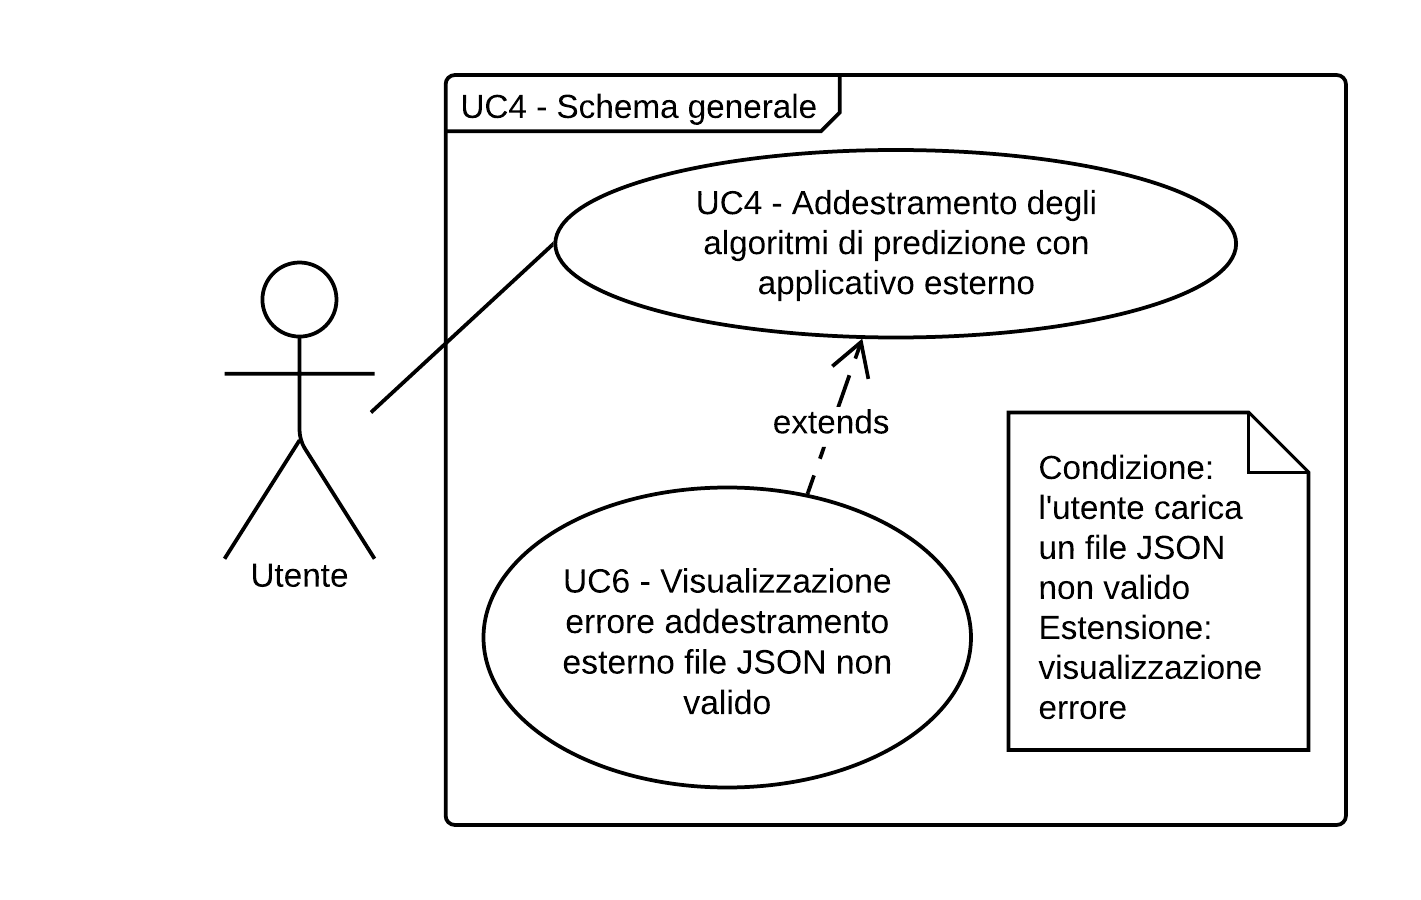
\includegraphics{img/UC4_-_Schema_generale.png}
\caption{Schema generale di UC4}
\end{figure}
\subsection{UC4 - Addestramento degli algoritmi di predizione con applicativo esterno}
\begin{figure}[H]
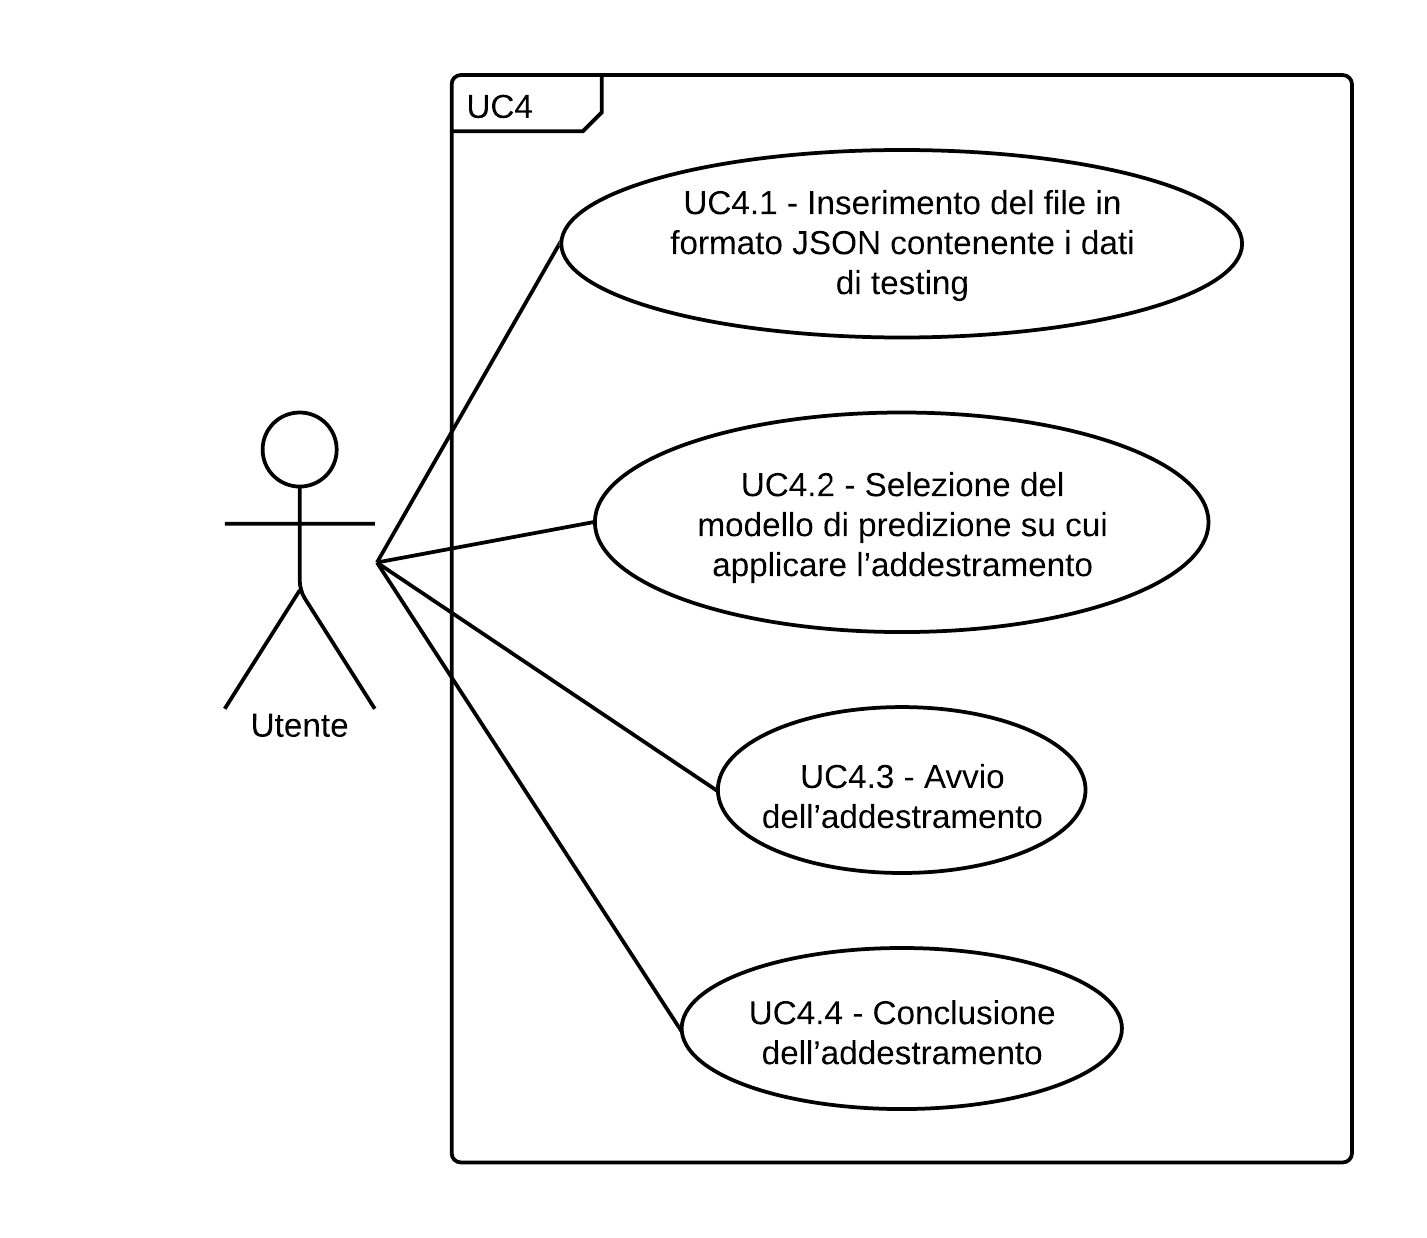
\includegraphics{img/UC4_-_Addestramento_degli_algoritmi_di_predizione_con_applicativo_esterno.png}
\caption{Diagramma degli use case di UC4}
\end{figure}
\begin{itemize}
    \item \textbf{Codice identificativo}: UC4;
    \item \textbf{Titolo}: Addestramento degli algoritmi di predizione con applicativo esterno;
    \item \textbf{Attori primari}: Utente;
    \item \textbf{Descrizione}: Attività di addestramento degli algoritmi di predizione eseguita nell'applicativo esterno a Grafana\glosp utilizzando dei dati inseriti da un utente;
    \item \textbf{Precondizioni}: L'utente è autenticato nel sistema software Grafana\glo;
    \item \textbf{Postcondizioni}: L'utente ha completato l'addestramento degli algoritmi di predizione;
    \item \textbf{Scenario principale}: 
        \begin{enumerate}
            \item Inserimento del file in formato JSON contenente i dati di testing (UC4.1);
            \item Selezione del modello di predizione su cui applicare l'addestramento (UC4.2);
            \item Avvio dell'addestramento (UC4.3);
            \item Conclusione dell'addestramento (UC4.4);
            \item Ricezione del file JSON (UC4.5). 
        \end{enumerate}
    \item \textbf{Estensioni}:
    \begin{itemize}
    	\item Se il caricamento del file JSON non è avvenuto con successo viene visualizzato un messaggio di errore (UC6).
    \end{itemize}
\end{itemize}

\subsubsection{UC4.1 - Inserimento del file in formato JSON contenente i dati di testing}
\begin{figure}[H]
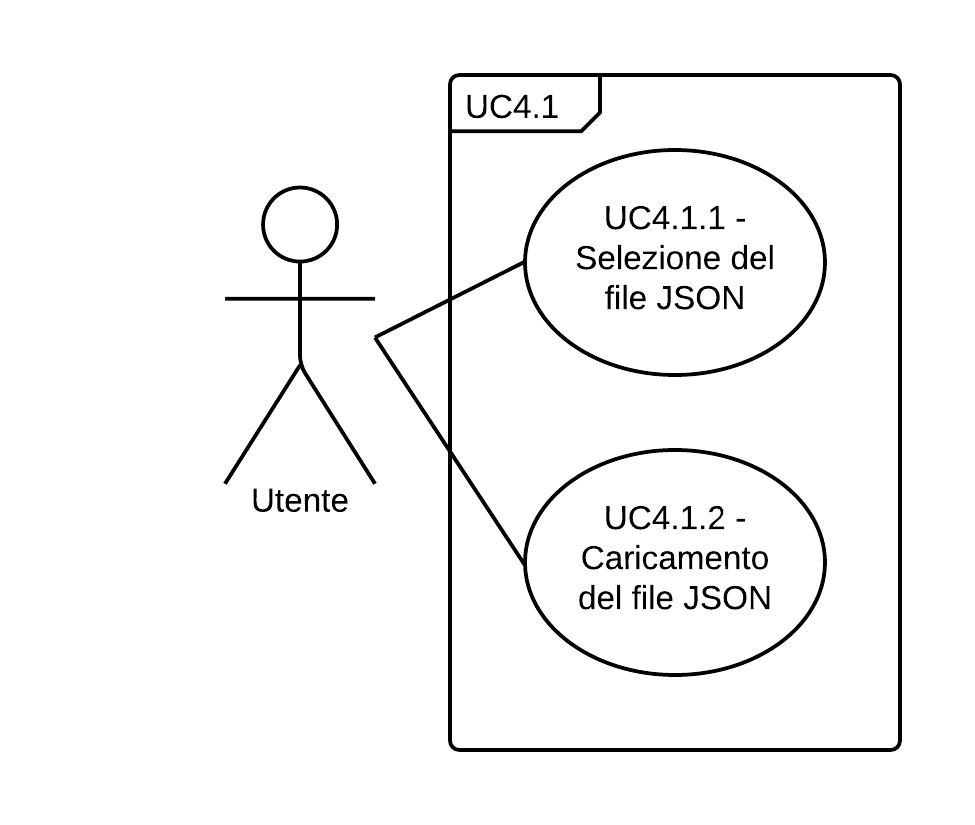
\includegraphics{img/UC4.1_-_Inserimento_del_file_in_formato_JSON_contenente_i_dati_di_testing.png}
\caption{Diagramma degli use case di UC4.1}
\end{figure}
\begin{itemize}
    \item \textbf{Codice identificativo}: UC4.1;
    \item \textbf{Titolo}: Inserimento del file in formato JSON contenente i dati di testing;
    \item \textbf{Attori primari}: Utente;
    \item \textbf{Descrizione}: L'utente inserisce un file in formato JSON contenente i dati di testing nell'applicazione esterna;
    \item \textbf{Precondizioni}: L'utente è autenticato nel sistema software Grafana\glo;
    \item \textbf{Postcondizioni}: L'utente ha inserito correttamente il file JSON;
    \item \textbf{Scenario principale}:
		\begin{enumerate}
			\item Selezione del file JSON (UC4.1.1);
			\item Caricamento del file JSON (UC4.1.2).
		\end{enumerate}
\end{itemize}

\paragraph{UC4.1.1 - Selezione del file JSON}
\begin{itemize}
	\item \textbf{Codice identificativo}: UC4.1.1;
	\item \textbf{Titolo}: Selezione del file JSON;
	\item \textbf{Attori primari}: Utente;
	\item \textbf{Descrizione}: L'utente seleziona il file JSON da inserire nell'applicativo esterno;
	\item \textbf{Precondizioni}: L'utente è autenticato nel sistema software Grafana\glo;
	\item \textbf{Postcondizioni}: L'utente ha selezionato correttamente il file JSON;
	\item \textbf{Scenario principale}: L'utente seleziona il file JSON.
\end{itemize}

\paragraph{UC4.1.2 - Caricamento del file JSON}
\begin{itemize}
	\item \textbf{Codice identificativo}: UC4.1.2;
	\item \textbf{Titolo}: Caricamento del file JSON;
	\item \textbf{Attori primari}: Utente;
	\item \textbf{Descrizione}: L'utente carica il file JSON nell'applicativo esterno;
	\item \textbf{Precondizioni}: L'utente ha selezionato il file da caricare;
	\item \textbf{Postcondizioni}: L'utente ha caricato correttamente i file JSON;
	\item \textbf{Scenario principale}: L'utente carica il file JSON.
\end{itemize}

\subsubsection{UC4.2 - Selezione del modello di predizione su cui applicare l'addestramento}
\begin{itemize}
    \item \textbf{Codice identificativo}: UC4.2;
    \item \textbf{Titolo}: Selezione del modello di predizione su cui applicare l'addestramento;
    \item \textbf{Attori primari}: Utente;
    \item \textbf{Descrizione}: L'utente seleziona quale modello di predizione applicare durante l'addestramento;
    \item \textbf{Precondizioni}: Il file JSON è stato inserito correttamente;
    \item \textbf{Postcondizioni}: Il modello di predizione è stato scelto correttamente;
    \item \textbf{Scenario principale}: L'utente seleziona un modello di predizione per eseguire l'addestramento.   
\end{itemize}

\subsubsection{UC4.3 - Avvio dell'addestramento}
\begin{itemize}
    \item \textbf{Codice identificativo}: UC4.3;
    \item \textbf{Titolo}: Avvio dell'addestramento;
    \item \textbf{Attori primari}: Utente;
    \item \textbf{Descrizione}: Viene fornito all'utente un modo per avviare l'addestramento;
    \item \textbf{Precondizioni}: Il file JSON è stato inserito correttamente e il modello di predizione è stato selezionato;
    \item \textbf{Postcondizioni}: L'addestramento è stato avviato con successo;
    \item \textbf{Scenario principale}: L'utente avvia l'addestramento.
\end{itemize}

\subsubsection{UC4.4 - Conclusione dell'addestramento}
\begin{figure}[H]
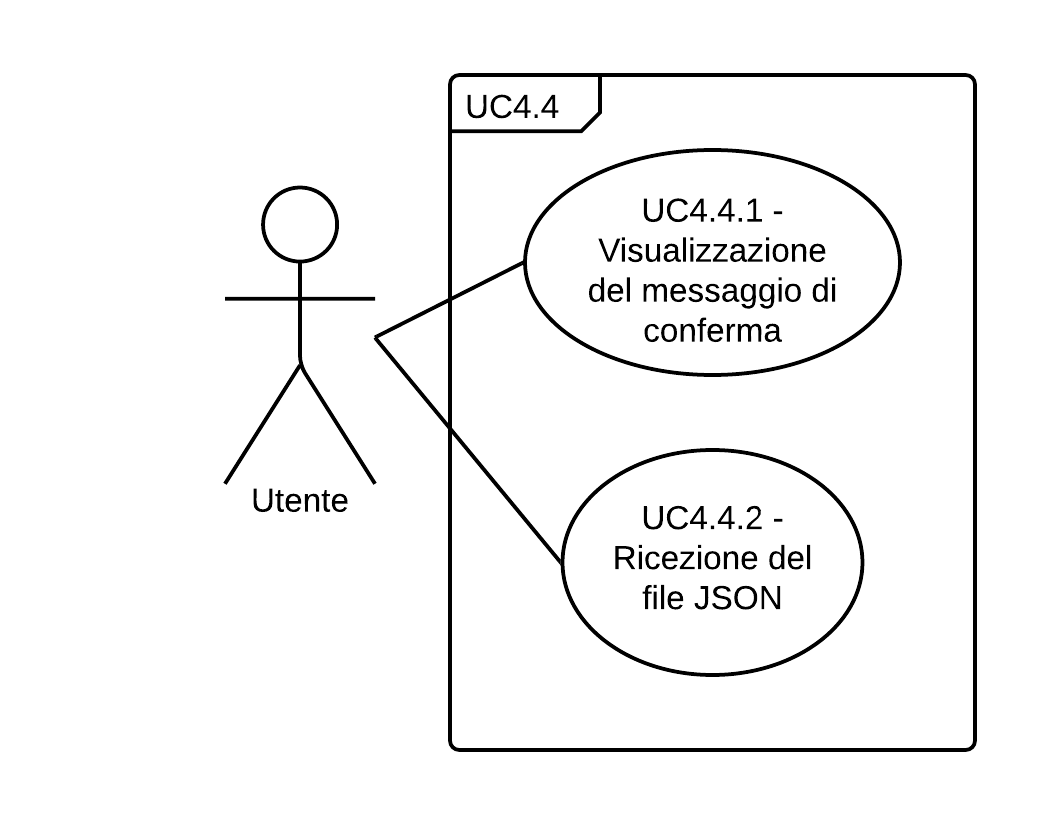
\includegraphics{img/UC4.4_-_Conclusione_dell_addestramento.png}
\caption{Diagramma degli use case di UC4.4}
\end{figure}
\begin{itemize}
    \item \textbf{Codice identificativo}: UC4.4;
    \item \textbf{Titolo}: Conclusione dell'addestramento;
    \item \textbf{Attori primari}: Utente;
    \item \textbf{Descrizione}: L'applicazione esterna ha concluso l'addestramento;
    \item \textbf{Precondizioni}: L'addestramento è stato avviato con successo;
    \item \textbf{Postcondizioni}: L'addestramento è stato concluso con successo;
    \item \textbf{Scenario principale}: L'utente visualizza un messaggio di conferma e conclude l'addestramento.
\end{itemize}

\paragraph{UC4.4.1 - Visualizzazione del messaggio di conferma}
\begin{itemize}
	\item \textbf{Codice identificativo}: UC4.4.1;
	\item \textbf{Titolo}: Visualizzazione del messaggio di conferma;
	\item \textbf{Attori primari}: Utente;
	\item \textbf{Descrizione}: L'utente visualizza un messaggio di conferma che l'addestramento è stato eseguito correttamente;
	\item \textbf{Precondizioni}: L'addestramento è stato avviato con successo;
	\item \textbf{Postcondizioni}: L'utente ha visualizzato un messaggio di conferma che l'addestramento è stato eseguito correttamente;
	\item \textbf{Scenario principale}: L'utente visualizza un messaggio di conferma che l'addestramento è stato eseguito correttamente.
\end{itemize}


\paragraph{UC4.4.2 - Ricezione del file JSON}
\begin{itemize}
    \item \textbf{Codice identificativo}: UC4.4.2;
    \item \textbf{Titolo}: Ricezione del file JSON;
    \item \textbf{Attori primari}: Utente;
    \item \textbf{Descrizione}: L'applicazione restituisce un file JSON con l'addestramento dei dati completato;
    \item \textbf{Precondizioni}: L'applicazione esterna ha concluso l'addestramento con successo;
    \item \textbf{Postcondizioni}: L'utente ha ricevuto il file JSON dei risultati dell'addestramento;
    \item \textbf{Scenario principale}: L'utente riceve il file JSON dei risultati dell'addestramento.
\end{itemize}